\documentclass{beamer}

\usepackage{lipsum}      % Use for dummy text, for instance \lipsum[1-4] prints 4 paragraphs

\mode<presentation>{\usetheme{Ringerike}} \usepackage[english]{babel} \usepackage[latin1]{inputenc}
\usepackage{siunitx}
\usepackage{subcaption}
\usepackage{multicol}
\usepackage{colortbl}
\usepackage{multirow}
\usepackage{tabularx}
\newcolumntype{C}{>{\centering\arraybackslash}X}

% \usepackage{amsmath,amsthm, amssymb, latexsym} \boldmath

% Size of poster
\usepackage[size=a0,orientation=portrait]{beamerposter}

\addtobeamertemplate{block begin}{}{\setlength{\parskip}{30pt plus 1pt minus 1pt}}
\setbeamertemplate{caption}[numbered]

% Bibliography colors and labels
\setbeamertemplate{bibliography item}{\color{white}\insertbiblabel}
\setbeamercolor{bibliography entry item}{fg=white}
\setbeamercolor{bibliography entry author}{fg=white}
\setbeamercolor{bibliography entry title}{fg=white} 
\setbeamercolor{bibliography entry location}{fg=white} 
\setbeamercolor{bibliography entry note}{fg=white}

\title{NMA Analysis Center}
\subtitle{Progress Report}
\author{Ann-Silje Kirkvik, Geir Arne Hjelle, {\AA}smund Skj{\ae}veland, Michael D\"ahnn, Ingrid Fausk}
\newcommand{\contact}{ann-silje.kirkvik@kartverket.no geir.arne.hjelle@kartverket.no asmund.skjaeveland@kartverket.no}
\institute{Norwegian Mapping Authority, Geodetic Institute}
\date{June 3-8, 2018}

\usebackgroundtemplate{
\includegraphics[width=\paperwidth]{figure/earth}}

\begin{document}
\begin{frame}[t]
  % Top title area
  \color{white} 
  \vspace*{2cm}
  \begin{columns}
    \begin{column}[t]{.97\textwidth}
      {\bfseries\fontsize{88}{120}\selectfont \inserttitle}
      {\fontsize{88}{120}\selectfont\kern2cm---\kern2cm\insertsubtitle}
    \end{column}
  \end{columns}

  \vspace*{2cm}
  \begin{columns}
    \begin{column}[t]{.25\textwidth}
      {\fontsize{30}{36}\selectfont\insertauthor\\[0.5cm]
        \fontsize{30}{36}\selectfont{\itshape\insertinstitute}\\
        \fontsize{24}{18}\selectfont\texttt{\contact}}
    \end{column}

    \begin{column}[t]{.7\textwidth}
      {\fontsize{30}{36}\selectfont\setlength{\parskip}{30pt}At the Norwegian Mapping Authority, we are currently developing Where, a new
software for geodetic analysis. Where is built on our experiences with the
Geosat software, and will be able to analyse and combine data from VLBI, SLR,
GNSS and DORIS. The software is mainly written in Python which has proved very
fruitful. The code is quick to write and the architecture is easily extendable
and maintainable, while at the same time taking advantage of well-tested libraries
like the SOFA and IERS packages.

At the moment the VLBI analysis is close to ready. Comparison to other softwares
show that theoretical delay computations in Where are consistent with those. SLR
and GNSS analysis is well under way.

\vspace*{-10cm}

\endinput
}
      \raisebox{0cm}{\kern52.5cm\color{white}\tiny PHOTO: GETTY IMAGES}
    \end{column}
  \end{columns}

  \begin{columns}

    % Content area
    \begin{column}[t]{.72\textwidth}
      \begin{block}{Norwegian Mapping Authority Analysis Center}
        \begin{multicols}{3}
          The Norwegian Mapping Authority has been an Associate Analysis Center within the IVS
(\cite{behrend2013}, \cite{schuh2012}) since 2010.  The original plan was to use the GEOSAT software~\cite{kierulf2010}
and become an operational analysis center which regularly processes R1 and R4 sessions. As previously reported in the
IVS 2015+2016 Biennial Report~\cite{kirkvik2017a}, the GEOSAT software was abandoned and a new software is under
development. The new software is called \textbf{Where} (Figure~\ref{fig:architecture}, \cite{kirkvik2017b}).  NMA plans
to use this software to submit timely analysis to the IVS combination center.

{\large\bfseries Motivation}\\

NMA has operated the VLBI station in Ny-{\AA}lesund since the beginning of the 1990s with the first observations in
1994. The site is currently being upgraded with two new VLBI stations and a SLR station is planned added to the site by
2022.  Several GNSS stations and a DORIS beacon already exist in Ny-{\AA}lesund.

Ny-{\AA}lesund is situated at \ang{78,55}N, \ang{11,56}E on the west coast of Spitsbergen, the largest island in the
Svalbard archipelago. Ny-{\AA}lesund is not open to the general public and professionals working there are limited to
fixed term contracts. This naturally causes a high turnover and finding qualified personnel for a small field of
science, such as VLBI and SLR, is a continuous challenge. Having qualified personnel in permanent positions at the head
office is therefore essential. Creating an analysis software provides valuable compentence and insights into the field
of VLBI for the group at the head office. Additionally -- by becoming an analysis center NMA can finally analyze the
data collected at Ny-{\AA}lesund and provide direct feedback to the station on its performance.

{\large\bfseries Software}\\

In 2017 the theoretical VLBI delay model of the \textbf{Where} software was confirmed to be comparable with other
software packages~\cite{kirkvik2017b}.  This was done by utilizing the data and analysis from the VLBI Analysis
Software Comparison Campaign~\cite{klopotek2016}.

\textbf{Where} uses a Kalman filter with a Modified Bryson-Frazier smoother (\cite{bierman2006}, \cite{gibbs2011})
for estimation.  Table \ref{tbl:sigmas} shows the default a priori covariance used.  Clocks and troposphere are
modelled as continuous piecewise linear parameters. The clocks and the wet troposphere are estimated with one linear
segment per hour, while the horizontal gradients use one linear segment per 6 hours. Normal equations as requested by
the IVS are created following the method of~\cite{mysen2017}.

The \textbf{Where} software is available under an open source MIT license at:\\[-10pt]
\begin{center}
\url{github.com/kartverket/where}
\end{center}

{\large\bfseries Status}\\

Lately, a lot of effort has been put into analyzing sessions from 1994 to 2016 to identify clock breaks and other
issues with the data. Furthermore, the estimation and writer components have been completed and a lot of testing has
been done.

In March 2018 the first test solution was submitted to the IVS combination center. It consisted of one year of sessions
(2016) and contained estimates for Earth Orientation Parameters (EOP) and station coordinates. Later, as solution with
23 years of processed sessions (1994-2016) was also submitted. The second solution also contained estimates for radio
source coordinates. These solutions were processed by the same modelling code.

However, there were some problems with the submitted solutions. First of all, the radio source names were wrong for
those sources that are listed in the observation file with a different name than the official IERS name. Work is
underway to fix this problem.

Secondly -- and more worrisome -- the estimates appeared to be extremely close to the a priori values. Since almost all
other VLBI analysis software packages apply a least squares estimator, the first suspicion was that too strong
constraints were being applied.  As it turned out, the problem was found elsewhere. The main problem was that when the
Kalman filter iterated and removed outliers it did not estimate the parameters from scratch, but rather estimated a
correction to the previous estimate. It was this correction to the previous estimate that was wrongly used to generate
the normal equations.  The first (and second) solution also contained large offsets in estimated station coordinates for
some stations and the computed weight factor for the solution in the combination was too low.

The implementation of the creation of the normal equations also contained some mistakes. All these mistakes were
corrected in a new version of the software. A third solution with station coordinates and EOPs using sessions from 2013
to 2016 was submitted. The station coordinates from NYALES20 from this third solution are plotted in
Figure \ref{fig:nyal}.

The magnitude of the estimates now seems to be reasonable and the estimates are no longer too optimistic. But they
are still slightly different from the other analysis centers and the combined solution. They appear to have the
opposite sign.  Some of the stations participated in too few sessions in the analyzed time span to be able to draw any
conclusions, but for instance the height component of NYALES20 fits well with this theory. See Figure~\ref{fig:nyal_h}.

In addition, the offsets observed in the previous solutions and the weight factor became worse instead of better. This
is probably also caused by having the wrong sign on the estimates.  Some initial inspection of the code suggest that
the wrong sign is caused by the sign of the residual vector, which is then also wrong. However, more sessions need to
be analyzed and tested in the combination before this theory can be confirmed.

There are also some problems with the EOPs. There is an offset in UT1-UTC and a large variability in the estimates for
most of the parameters compared to the other analysis centers. This needs to be investigated further after the sign
error has been fixed.

{\large\bfseries Time schedule}\\

The immediate plan is to continue to submit analyzed sessions to the IVS Combination Center to improve the quality of
the solution. When the estimates of station coordinates and the EOPs seem reasonable, the source coordinates will be
added again. 

When the quality is approved, the next step is to start analyzing regularly the R1 and R4 sessions and to
establish good routines for upholding the timeliness requirement. The plan is to start regular analysis by the end of
2018. This step will involve a different set of challenges such as automation of the analysis and having qualified
personnel available during vacations.

In addition, outliers should be studied more closely. Some sessions do not have enough usable observations to estimate
the full set of parameters. These sessions require special handling and complicates the road to automating the analysis
as much as possible.

\vspace*{15ex}

\endinput

        \end{multicols}
      \end{block}
    \end{column}

    \begin{column}[t]{.24\textwidth}
      \vspace*{7cm} % Align image row below headline of box to the left
        \begin{figure}
             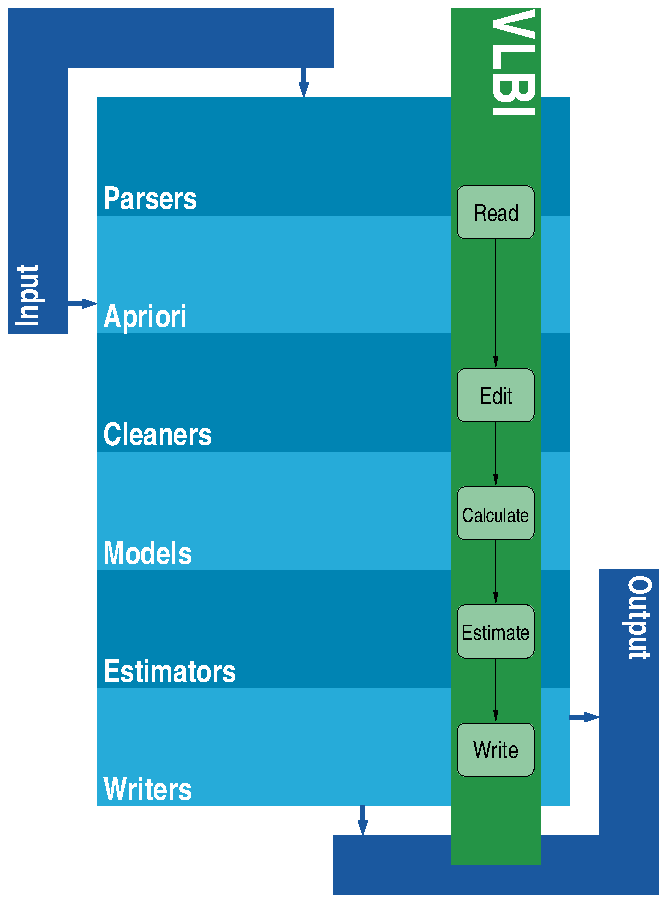
\includegraphics[width=\textwidth]{figure/code_structure_vlbi}
             \caption{\textbf{Where} architecture: The pipeline for the analysis of VLBI sessions.}
            \label{fig:architecture}
        \end{figure}

      \vspace*{2cm}     % Some space between image row and table
       \begin{table}
         \color{black}
\setlength{\extrarowheight}{10pt}
\begin{tabularx}{\columnwidth}{X|r}
\hline
\rowcolor{kvgreen}\textcolor{white}{\textbf{Parameter}} & \textcolor{white}{$\sigma$} \\
\hline
\multicolumn{2}{l}{\textbf{Constant parameters}} \\
\hline
Station coordinate      & 1\,m \\
UT1-UTC                 & 1\,ms \\
LOD                     & 1\,ms \\
Polar motion            & 1\,mas \\
Polar motion rate       & 1\,mas/d \\
Precession/Nutation     & 1\,mas \\
Radio source coordinate & $2.5\times 10^{-7}$\,rad \\
\hline
\multicolumn{2}{l}{\textbf{Piecewise Linear Parameters (offset and rate)}} \\
\hline
Clock                   & 1\,m and 1\,m/h\\
Wet troposphere         & 1\,m and 1\,m/h \\
Horizontal gradients    & 1\,m and 1\,m/h \\
\hline
\end{tabularx}

\endinput

         \caption{Default a priori covariance matrix used in \textbf{Where}. The matrix is a diagonal matrix with
         $\sigma^2$ on the diagonal.}
         \label{tbl:sigmas}
       \end{table}

     \end{column}
   \end{columns}


  % Figure strip
  \vspace*{1cm}
  \begin{columns}
    \begin{column}[t]{\textwidth}
     \begin{figure}
      \begin{subfigure}{0.33\textwidth}
        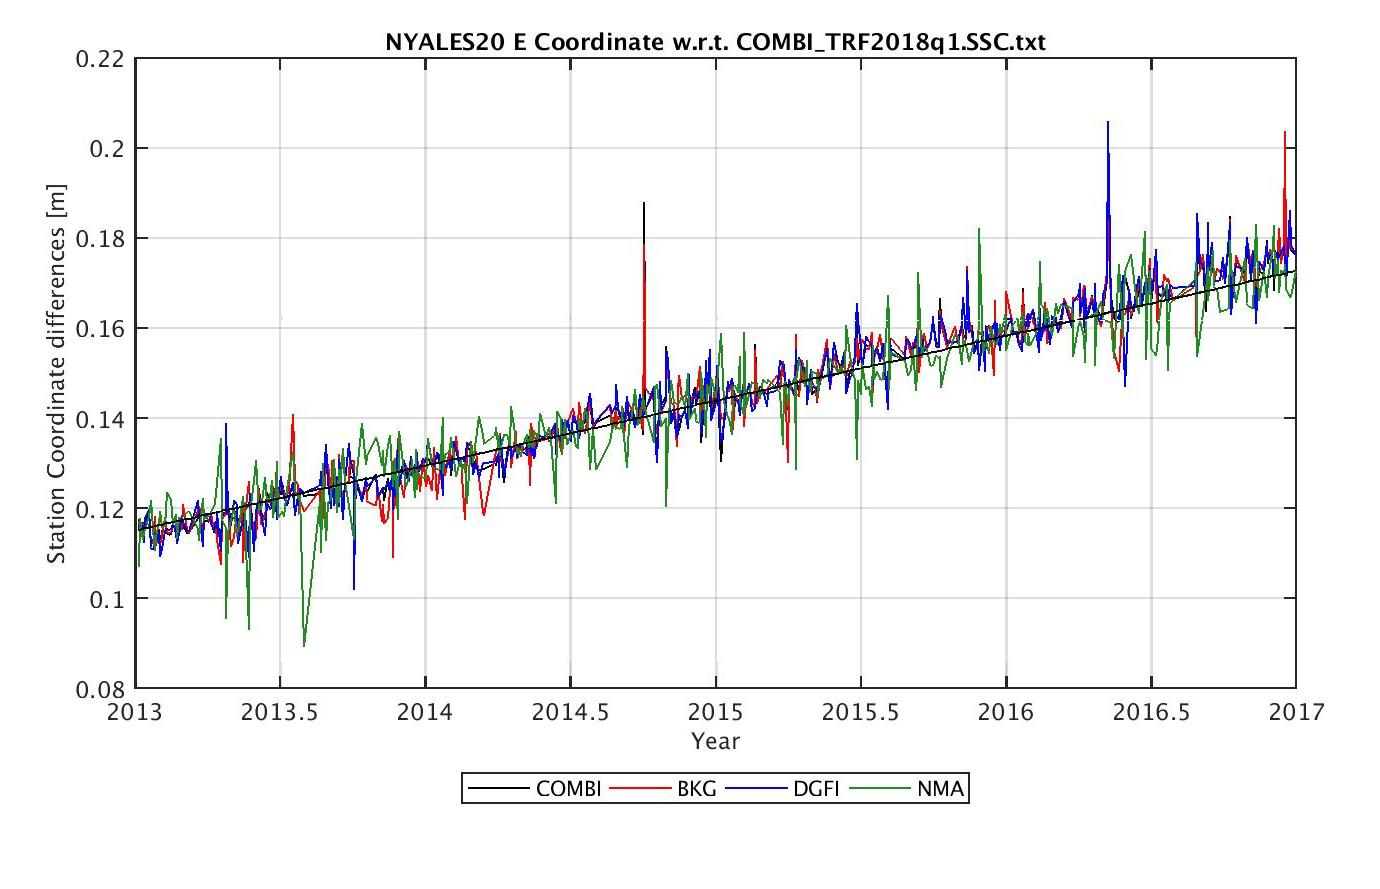
\includegraphics[width=\linewidth]{figure/NYALES20-E_diff-trf}
        \caption{East}
        \label{fig:nyal_e}
      \end{subfigure}
      \begin{subfigure}{0.33\textwidth}
        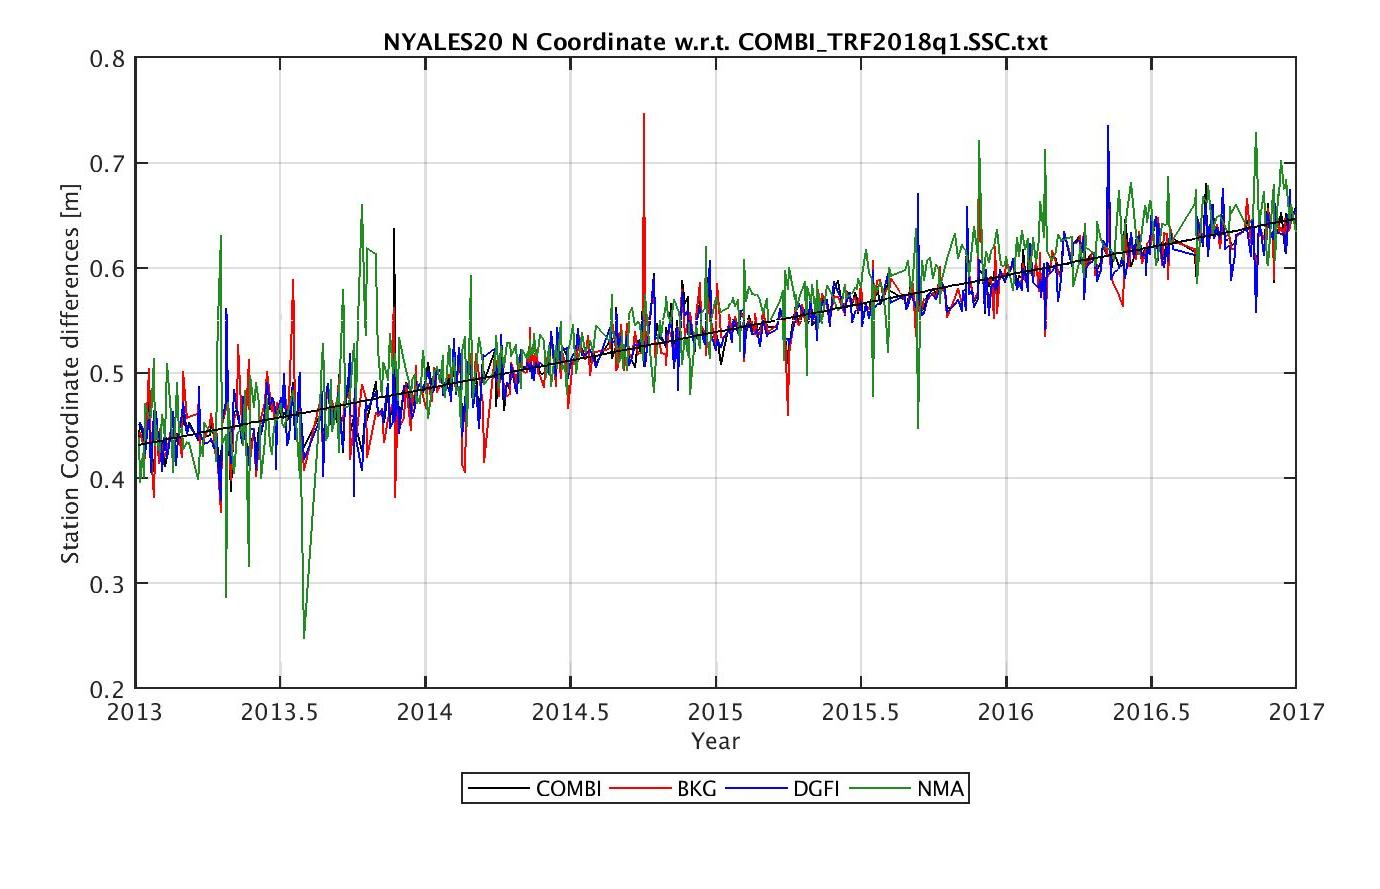
\includegraphics[width=\linewidth]{figure/NYALES20-N_diff-trf}
        \caption{North}
        \label{fig:nyal_n}
      \end{subfigure}
      \begin{subfigure}{0.33\textwidth}
        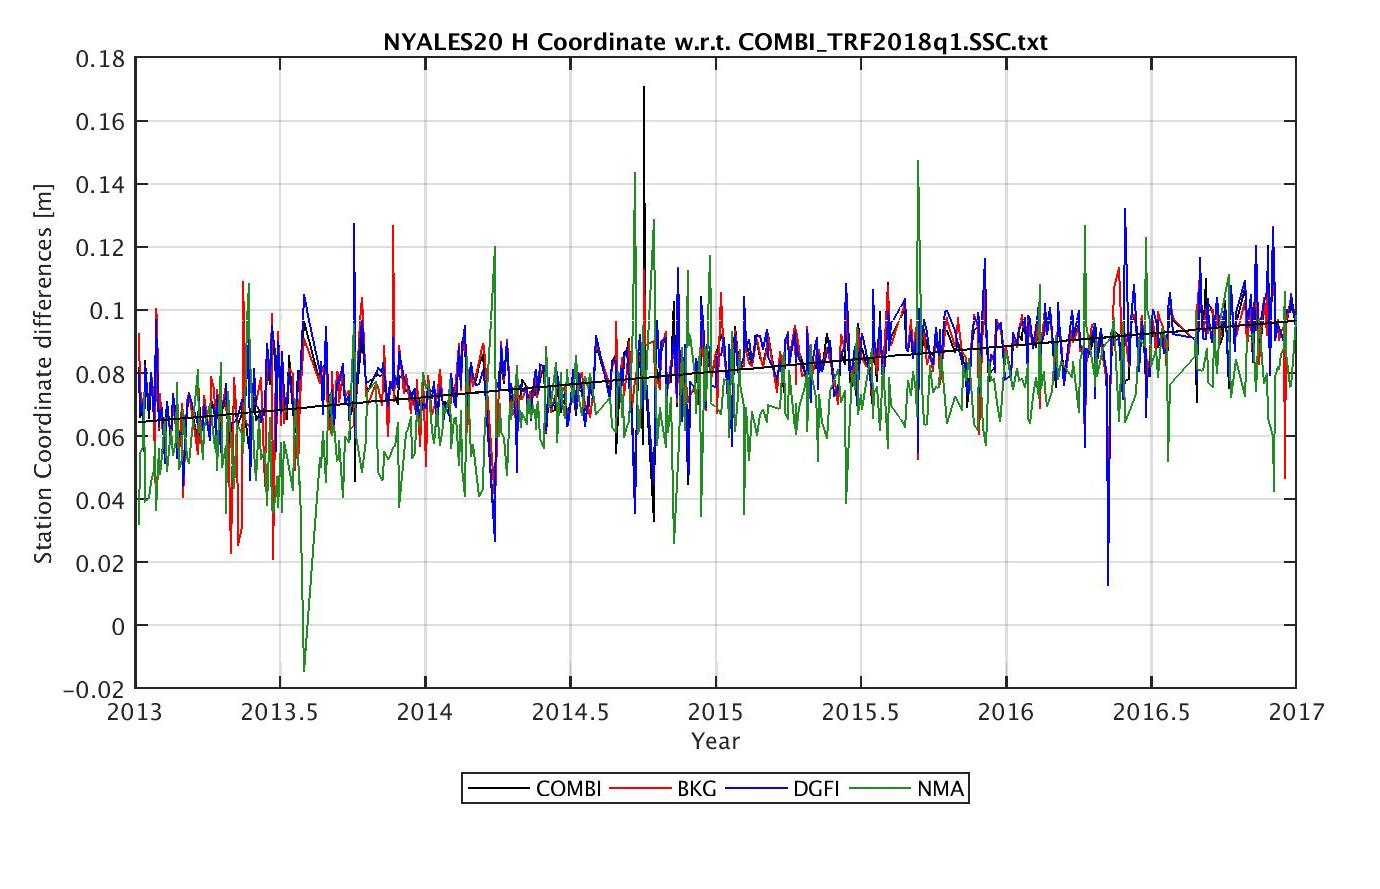
\includegraphics[width=\linewidth]{figure/NYALES20-H_diff-trf}
        \caption{Height}
        \label{fig:nyal_h}
      \end{subfigure}
      \caption{Difference between estimated station coordinates for NYALES20 and a reference frame solution for the
        third submission.  A few large outliers have been removed. Provided by Sabine Bachmann, BKG.}
      \label{fig:nyal}
      \end{figure}
    \end{column}
  \end{columns}

  % References box
  \vspace*{1cm}
  \begin{columns}
    \begin{column}[t]{.15\textwidth}
      % Spacing (for Kartverket logo)
    \end{column}

    \begin{column}[t]{.82\textwidth}
      \begin{block}{References and Acknowledgements}
        \vspace*{-1cm}                   % Too much space on top inside block
        \begin{minipage}{.98\textwidth}  % Add space left and right
          \begin{multicols}{4}
            \footnotesize
\bibliographystyle{../../where}
\bibliography{../../where}
\endinput

            %\columnbreak

            \vspace*{3ex}{\bfseries Acknowledgements}\\

            Thanks to Sabine Bachmann (BKG) at the IVS Combination Center for analyzing our solutions and providing great feedback and insights.
          \end{multicols}
        \end{minipage}
      \end{block}
    \end{column}
  \end{columns}
\end{frame}
\end{document}
